\documentclass[10pt]{article}
\usepackage[top=2.5cm, bottom=3cm, left=2.3cm, right=2.3cm]{geometry}
\usepackage{graphicx}
\usepackage{subfigure}
\usepackage{psfrag}
\usepackage{amsmath}
\usepackage{natbib}
\usepackage{color}
\usepackage[normalem]{ulem}
\usepackage{csquotes}
\usepackage{cleveref}
\usepackage{epstopdf, epsfig}
\usepackage{wrapfig}
\usepackage{amsbsy}
\usepackage{lineno,hyperref}
\usepackage{verbatim}
\usepackage{tikz}
\usepackage[makeroom]{cancel}

\tikzset{math/.style={draw, execute at begin node={$\displaystyle}, execute at end node={$}}}

\newcommand{\boxandcomment}[4][]{%
    \tikz[baseline=(#2.base), remember picture]{%
        \node[math, label=below:{#3}, #1] (#2) {#4};}}

\newcommand{\norm}[1]{\left\lVert#1\right\rVert}
\def\lp{\left(}
\def\rp{\right)}
\def\tp{\overline{{\theta^\prime}^2}}
\def\tm{\overline{\theta}}
\def\tr{{\theta^\prime}}
\def\et{{\varepsilon_{\theta}}}

\begin{document}
\section*{Radiative modification to a general $\overline{u_j^\prime \tr}$ model}
\vspace{1cm}
Radiative heat transfer modifies intrinsically the turbulent temperature field, modifying the mechanism of turbulent heat transfer (TRI). This leads to an average temperature profile that cannot be predicted with standard models. Therefore, hereby we extend a classical two equation model (temperature variance - dissipation of temperature variance) to account for TRI. The two equation model is chosen because of its simplicity and reliability but the general guidelines laid down in this first section are general and applicable to any turbulent heat flux model. \\
TRI is driven by the the appearence of a fluctuating radiative field, therefore the quantities requiring modeling are:

\begin{equation*}
\kappa^\prime \ , \ \ \ E_m^\prime \ , \ \ \ G^\prime \ .
\end{equation*}
They all depend on temperature (Radiative heat transfer is an analytical equation), in particular we know that:
\begin{equation*}
\kappa = c_0 + \frac{c_1}{T} + \frac{c_2}{T^2} + \frac{c_3}{T^3} + \frac{c_4}{T^4} + \frac{c_5}{T^5} \ ,
\end{equation*}
and
\begin{equation*}
E_m = 4 {\lp \frac{\theta}{T_0} + 1\rp }^4 \ ,
\end{equation*}
where:
\begin{equation*}
T = \theta \Delta T + T_c \ ,  \ \ \ \ \overline{T} = \tm \Delta T+ T_c \ , \ \ \ \ T^\prime = \tr \Delta T \ , \ \ \ \ T_0 = \frac{T_c}{\Delta T} \ .
\end{equation*}
\subsection*{Approximation of $E_m^\prime$}
It is possible to find the fluctuation of these two quantities by linearizing their analytical expressions, starting from $E_m$
\begin{equation*}
E_m^\prime  = E_m - \overline{E}_m = 4 {\lp \frac{\theta}{T_0} + 1\rp }^4 - 4\overline{ {\lp \frac{\theta}{T_0} + 1\rp }^4}
\end{equation*}
\begin{equation*}
E_m^\prime  = \frac{4 \theta^4}{T_0^4} + \frac{16 \theta^3}{T_0^3} + \frac{24 \theta^2}{T_0^2} + \frac{16\theta}{T_0}  
            - \frac{4 \overline{\theta^4}}{T_0^4} - \frac{16 \overline{\theta^3}}{T_0^3} - \frac{24 \overline{\theta^2}}{T_0^2} - \frac{16\tm}{T_0}  
\end{equation*}
after subtituting $\theta$ with $\tr+\tm$
\begin{equation*}
\begin{split}
E_m^\prime & = \frac{4 (\tm^4 + 4\tm^3 \tr + 6\tm^2 \tr^2+4\tm\tr^3+\tr^4)}{T_0^4} + \frac{16 (\tm^3 + 3\tm^2\tr+3\tm\tr^2+\tr^3)}{T_0^3} + \frac{24 (\tm^2+2\tm\tr+\tr^2)}{T_0^2} + \frac{16(\tm+\tr)}{T_0} + \\
           & - \frac{4 (\tm^4 + 6\tm^2 \tp +4\tm\overline{\tr^3} + \overline{\tr^4})}{T_0^4} - \frac{16(\tm^3 +3\tm\tp+\overline{\tr^3})}{T_0^3} - \frac{24 \tm^2 + \tp}{T_0^2} - \frac{16\tm}{T_0}  \ ,
\end{split}
\end{equation*}
\begin{equation*}
\begin{split}
E_m^\prime & = \frac{4 (4\tm^3 \tr + 6\tm^2 (\tr^2-\tp)+4\tm(\tr^3-\overline{\tr^3})+\tr^4-\overline{\tr^4})}{T_0^4} + \frac{16 (3\tm^2\tr+3\tm(\tr^2-\tp)+\tr^3-\overline{\tr^3})}{T_0^3} + \\
           & + \frac{24 (2\tm\tr+\tr^2-\tp)}{T_0^2} + \frac{16(\tr)}{T_0}  \ .
\end{split}
\end{equation*}
In the end, simplifying and underlying the dependency on temperature fluctuations $\tr$:
\begin{equation*}
\begin{split}
E_m^\prime & = \lp \frac{16 \tm^3}{T_0^4} + \frac{48 \tm^2}{T_0^3} + \frac{48 \tm}{T_0^2} + \frac{16}{T_0}  \rp \tr + \\
           & = \lp \frac{24 \tm^2}{T_0^4} + \frac{48 \tm}{T_0^3}   + \frac{24}{T_0^2}   \rp (\tr^2 - \tp) + \\
           & = \lp \frac{16 \tm}{T_0^4}   + \frac{16} {T_0^3}   \rp (\tr^3 - \overline{\tr^3}) + \\
           & = \lp \frac{4}{T_0^4}  \rp (\tr^4 - \overline{\tr^4})  \ .
\end{split}
\end{equation*}
Due to the linearization we can neglect all terms depending on higher order terms, therefore in the end a good approximation for $E_m^\prime$ is
\begin{equation*}
E_m^\prime \approx f_{E_m} \theta^\prime \ ,
\end{equation*}
where $f_{E_m}$ is the first model equation, equal to:
\begin{equation*}
f_{E_m} =  \frac{16 \tm^3}{T_0^4} + \frac{48 \tm^2}{T_0^3} + \frac{48 \tm}{T_0^2} + \frac{16}{T_0} \ .
\end{equation*}

\subsection*{Approximation of $\kappa^\prime$ (only for variable $\kappa$)}
To calculate $\kappa^\prime$ is necessary to calculate $\overline{\kappa}$ first as $\kappa^\prime = \kappa - \overline{\kappa}$.
\begin{equation*}
\overline{\kappa} = c_0 + \overline{\frac{c_1}{T}} + \overline{\frac{c_2}{T^2}} + \overline{\frac{c_3}{T^3}} + \overline{\frac{c_4}{T^4}} + \overline{\frac{c_5}{T^5}} \ ,
\end{equation*}
taking into account the second term on the LHS, (remembering that $c_1$ is a constant):
\begin{equation*}
\overline{\frac{1}{T}} = \overline{\frac{1}{\overline{T}(1+\frac{T^\prime}{\overline{T}})}} \ ,
\end{equation*}
since $T^\prime/\overline{T} \ll 1$ it is possible taking a taylor expansion ${(1+x)^{-1} = 1-x+x^2-x^3 ...}$ and linearize, therefore:
\begin{equation*}
\overline{\frac{1}{T}} \approx \overline{\frac{1}{\overline{T}}(1 - \frac{T^\prime}{\overline{T}})} = \frac{1}{\overline{T}} \ .
\end{equation*}
Proceding with the same logic it is possible to show that, if $T^\prime/\overline{T} \ll 1$, then:
\begin{equation*}
\overline{\frac{1}{T^2}} \approx \frac{1}{\overline{T^2}} \ , \ \ \ \overline{\frac{1}{T^3}} \approx \frac{1}{\overline{T^3}} \ , \ \ \ \overline{\frac{1}{T^4}} \approx \frac{1}{\overline{T^4}} \ , \ \ \ \overline{\frac{1}{T^5}} \approx \frac{1}{\overline{T^5}} \ .  
\end{equation*}
Therefore
\begin{equation*}
\overline{\kappa} \approx c_0 + \frac{c_1}{\overline{T}} + \frac{c_2}{\overline{T^2}} + \frac{c_3}{\overline{T^3}} + \frac{c_4}{\overline{T^4}} + \frac{c_5}{\overline{T^5}} \ .
\end{equation*}
To calculate $\kappa^\prime$ we start from the second term on the LHS
\begin{equation*}
c_1 \lp \frac{1}{T} - \frac{1}{\overline{T}} \rp = c_1 \lp \frac{\overline{T} - T}{T\overline{T}} \rp \ .
\end{equation*}
Substituting the expressions $T^\prime  = T - \overline{T} = \theta^\prime \Delta T$ and linearizing the denominator ($T\overline{T} \approx \overline{T}^2$)
\begin{equation*}
c_1 \lp \frac{1}{T} - \frac{1}{\overline{T}} \rp \approx - c_1 \frac{\Delta T}{\overline{T}^2} \tr \ .
\end{equation*}
For the third term, subtracting and expanding into $\overline{T}+T^\prime$
\begin{equation*}
c_2 \lp \frac{1}{T^2} - \frac{1}{\overline{T^2}} \rp = c_2 \lp \frac{\overline{{T^\prime}^2} - 2\overline{T}{T^\prime} - {T^\prime}^2}{(\overline{T}^2 + 2\overline{T}T^\prime + {T^\prime}^2)(\overline{T}^2 + \overline{{T^\prime}^2)}} \rp \ .
\end{equation*}
Again linearizing the denominator ($\approx \overline{T}^4$) and the numerator ($\approx 2\overline{T}T^\prime$) we reach
\begin{equation*}
c_2 \lp \frac{1}{T^2} - \frac{1}{\overline{T^2}} \rp \approx - c_2  \frac{2\Delta T}{\overline{T}^3} \tr \ .
\end{equation*}
In the same fashion it is possible to demonstrate that 
\begin{equation*}
\begin{split}
c_3 \lp \frac{1}{T^3} - \frac{1}{\overline{T^3}} \rp & \approx - c_3  \frac{3\Delta T}{\overline{T}^4} \tr \ ,\\
c_4 \lp \frac{1}{T^4} - \frac{1}{\overline{T^4}} \rp & \approx - c_4  \frac{4\Delta T}{\overline{T}^5} \tr \ ,\\
c_5 \lp \frac{1}{T^5} - \frac{1}{\overline{T^5}} \rp & \approx - c_5  \frac{5\Delta T}{\overline{T}^6} \tr \ .
\end{split}
\end{equation*}
And therefore we found an expression for $\kappa^\prime$ as
\begin{equation*}
\kappa^\prime \approx f_{\kappa} \theta^\prime \ ,
\end{equation*}
where
\begin{equation*}
f_{\kappa} =  - \lp c_1  \frac{\Delta T}{\overline{T}^2} + c_2  \frac{2\Delta T}{\overline{T}^3} + c_3  \frac{3\Delta T}{\overline{T}^4} +  c_4  \frac{4\Delta T}{\overline{T}^4} +  c_5  \frac{5\Delta T}{\overline{T}^6} \rp \ .
\end{equation*}
Of course if $\kappa$ is another function of temperature the expression of $f_{\kappa}$ will have to be adapted.
\subsection*{Approximation of $G^\prime$}
This is the most complex part of the modeling and requires the knowledge of the spectral wavenumbers of the non-radiative channel flow. It is possible to know only the spectral dependency of the incident radiation fluctuations, and in homogeneous isotropic turbulence for grey gas is
\begin{equation*}
\widehat{G^\prime} = \frac{\kappa}{\omega} \text{atan}\lp\frac{\omega}{\kappa} \rp \widehat{E_m^\prime} \ .
\end{equation*} 
From this it is already possible to state, following from the previous considerations on $E_m^\prime$, that
\begin{equation*}
\widehat{G^\prime} \approx \frac{\kappa}{\omega} \text{atan}\lp\frac{\omega}{\kappa} \rp f_{E_m} \widehat{\tr} \ .
\end{equation*}
The above equation states that the modes of $G^\prime$ are connected to the modes of $\tr$ depending on the wavenumber and on the absorption coefficient. This means that the higher the absorption coefficient the stronger $G^\prime$ gets and always on smaller $\omega$. It is possible to translate this proportionality to physical space if there is the knowledge of a charateristic wavenumber for which it is possible to write
\begin{equation*}
G^\prime \approx f_G f_{E_m} \theta^\prime
\end{equation*}
where 
\begin{equation*}
f_G = \frac{\kappa}{\omega_c} \text{atan}\lp\frac{\omega_c}{\kappa} \rp
\end{equation*}
and $\omega_c$ is a charateristic wavenumber that represents the integral wavenumber weighted on the energy spectrum at a certain $y-$location calculated as
\begin{equation*}
\omega_c = {\norm{\int_{0}^{\infty} \boldsymbol{\omega^\prime} E_{\theta}(\boldsymbol{\omega^\prime}) d \boldsymbol{\omega^\prime} / \int_0^{\infty} E_{\theta}(\boldsymbol{\omega^\prime}) d \boldsymbol{\omega^\prime}}}_2
\end{equation*}
This wavenumber should take into account the penalty of anisotropicity on the growth of $G^\prime$, i.e. there should be weights in the norm that promote the spectral direction which contains energy at the largest wavenumbers since radiative energy will most likely escape from those directions. For the present case, with DNS knowledge of the spectral redistribution of energy in the channel, it is identified that the spanwise spectral wavenumber is dominant over the streamwise (i.e., energy at larger wavenumbers) and we assume that the wall normal direction contains energy at the same wavenumbers that the spawise direction. Therefore, following the spectral energy redistribution noticed in figure \ref{spectra}, it is possible to approximate the charateristic wavenumber as a parabola (shape of energy redistribution in spanwise direction) as
\begin{equation*}
\omega_c = (c_{r33} - c_{r22}) y^2 - 2(c_{r33} - c_{r22})y +c_{r33} \ ,
\end{equation*}
with $c_{r33}$ and $c_{r22}$ the wavenumber of maximum energy at the walls and in the middle of the channel respectively. 

%\begin{figure}[htb]
%\centering
%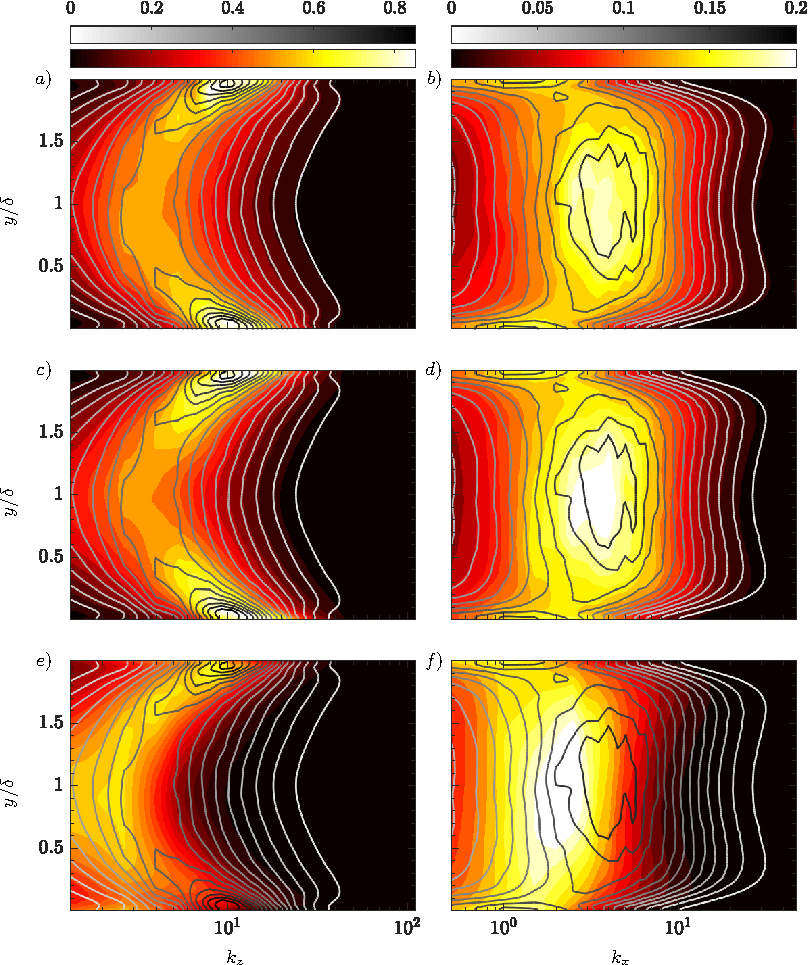
\includegraphics[width=1.1\textwidth]{fig13.pdf}
%\caption{\noindent Energy redistribution in the channel for turbulent temperature field from DNS simulations}
%\label{spectra}
%\end{figure}


\newpage
\section*{Modification of the $\tp - \varepsilon_{\theta}$ two equation model}
From the expressions derived in the previous section it is possible to extend a general $\tp-\varepsilon_{\theta}$ model to fit radiative flows. The two additional equations read:
\begin{equation}
\label{t2eq}
\frac{\partial \tp}{\partial t} + \overline{u}_j\frac{\partial \tp}{\partial x_j} = \frac{\partial}{\partial x_j} \lp \alpha \frac{\partial \tp}{\partial x_j} - \overline{u_j^\prime \tr^2} \rp - 2 \overline{u_j^\prime \tr} \frac{\partial \tm}{\partial x_j} - 2 \alpha \overline{\frac{\partial \tr}{\partial x_j}\frac{\partial \tr}{\partial x_j}} - \boxandcomment{X}{Radiative term $\mathcal{R}_{\tp}$}{2 \frac{\alpha}{\lambda}\overline{{(\kappa Q)}^\prime \tr}}
\end{equation}
\begin{equation}
\label{eteq}
\begin{split}
\frac{\partial \et}{\partial t} & + \overline{u}_j \frac{\partial \et}{\partial x_j}  =  \frac{\partial}{\partial x_j} \lp \alpha \frac{\partial \et}{\partial x_j} - \overline{u_j^\prime \et}  \rp - 2 \alpha \overline{\frac{\partial \tr}{\partial x_k} \frac{\partial u_j^\prime}{\partial x_k}} \frac{\partial \tm}{\partial x_j} - 2\alpha \overline{u_j^\prime \frac{\partial \tr}{\partial x_k}}\frac{\partial^2 \tm}{\partial x_j \partial x_k} \\
&- 2\alpha \overline{\frac{\partial \tr}{\partial x_k} \frac{\partial \tr}{\partial x_j}}\frac{\partial \overline{u}_j}{\partial x_k}  - 2 \alpha \overline{\frac{\partial \tr}{\partial x_k} \frac{\partial u_j^\prime}{\partial x_k}\frac{\partial \tr}{\partial x_j}} - 2\overline{{\alpha \frac{\partial^2 \tr}{\partial x_j \partial x_k}}^2} - \boxandcomment{Y}{Radiative term $\mathcal{R}_{\et}$}{2\frac{\alpha}{\lambda} \overline{\frac{\partial {(\kappa Q)}^\prime}{\partial x_k} \frac{\partial \tr}{\partial x_k}}}
\end{split}
\end{equation}
where $\et = \overline{\frac{\partial \tr}{\partial x_j}\frac{\partial \tr}{\partial x_j}}$ and $Q = E_m - G$. \\
The two equations contain the two additional \enquote{Radiative terms} which are unclosed terms and need to be modelled following the considerations done in the above section regarding $\kappa^\prime, \ E_m^\prime$ and $G^\prime$. Starting from equation (\ref{t2eq}), the additional term reads
\begin{equation*}
\mathcal{R}_{\tp} = 2\frac{\alpha}{\lambda} \lp \overline{\kappa} (\overline{E_m^\prime \tr}-\overline{G^\prime \tr}) + (\overline{E}_m - \overline{G})\overline{\kappa^\prime \tr} + \overline{\kappa^\prime E_m^\prime \tr} - \overline{\kappa^\prime G^\prime \tr} \rp
\end{equation*}
The last two terms on the LHS are third order terms and much smaller than the others, and a re therefore neglected. Following from the modelling of radiative fluctuations
\begin{equation*}
\mathcal{R}_{\tp} = 2\frac{\alpha}{\lambda} \lp \overline{\kappa} f_{E_m}(1 - f_G ) + (\overline{E}_m - \overline{G})f_{\kappa} \rp \tp
\end{equation*}
If $\kappa$ is constant $f_{\kappa} = 0$.\\
For equation (\ref{eteq}) the radiative term can be expanded as
\begin{equation*}
\mathcal{R}_{\et} = 2\frac{\alpha}{\lambda} \underbrace{ \lp \overline{\frac{\partial \kappa^\prime \overline{Q}}{\partial x_j}\frac{\partial \tr}{\partial x_j}}+\cancelto{\text{\tiny{linearize}}}{\overline{\frac{\partial \kappa^\prime Q^\prime}{\partial x_j}\frac{\partial \tr}{\partial x_j}}}\rp}_{\text{fluctuating }\kappa } + 2\frac{\alpha}{\lambda} \underbrace{ \lp \overline{\frac{\partial \overline{\kappa} Q^\prime}{\partial x_j}\frac{\partial \tr}{\partial x_j}} \rp}_{\text{average } \kappa }  
\end{equation*}
\begin{equation*}
\mathcal{R}_{\et} = 2\frac{\alpha}{\lambda} \lp \overline{\frac{\partial \kappa^\prime}{\partial x_j}\frac{\partial \tr}{\partial x_j}}\overline{Q} +\overline{\kappa^\prime\frac{\partial \tr}{\partial x_j}} \frac{\partial \overline{Q}}{\partial y}\rp + 2\frac{\alpha}{\lambda} \lp \overline{ Q^\prime\frac{\partial \tr}{\partial x_j}}\frac{\partial \overline{\kappa}}{\partial y}  +
 \overline{\frac{\partial Q^\prime}{\partial x_j}\frac{\partial \tr}{\partial x_j}}\overline{\kappa} \rp  
\end{equation*}
By substituting $\kappa^\prime = f_{\kappa} \tr$, $\overline{Q} = \overline{E}_m - \overline{G}$ and $Q^\prime = f_{E_m}(1-f_G) \tr$ we obtain


\begin{equation*} 
\begin{split}
\overline{\frac{\partial \kappa^\prime}{\partial x_j}\frac{\partial \tr}{\partial x_j}}\overline{Q} & = (\overline{E}_m-\overline{G}) \lp f_{\kappa} \et + \frac{1}{2}\frac{\partial f_{\kappa}}{\partial y}\frac{\partial \tp}{\partial y} \rp \\
\overline{\kappa^\prime\frac{\partial \tr}{\partial x_j}} \frac{\partial \overline{Q}}{\partial y} & = \frac{\partial (\overline{E}_m - \overline{G})}{\partial y} \frac{f_{\kappa}}{2} \frac{\partial \tp}{\partial y} \\
\overline{ Q^\prime\frac{\partial \tr}{\partial x_j}}\frac{\partial \overline{\kappa}}{\partial y} & = \frac{\partial \overline{\kappa}}{\partial y} \frac{f_{E_m}(1-f_G)}{2}\frac{\partial \tp}{\partial y}\\
\overline{\frac{\partial Q^\prime}{\partial x_j}\frac{\partial \tr}{\partial x_j}}\overline{\kappa} & = \overline{\kappa} \lp f_{E_m}(1-f_G) \et + \frac{1}{2}\frac{\partial f_{Em}(1-f_G)}{\partial y} \frac{\partial \tp}{\partial y} \rp
\end{split}
\end{equation*}

\noindent \textcolor{red}{Unfortunately we use only two of the above terms (namely term 1 and term 4) because term 2 and 3 are unstable. I still need to find an explanation for this.}


\noindent Both $\tp$ and $\et$ are required for the calculation of $\alpha_t$ which approximates $\overline{v^\prime \tr}$ as
\begin{equation*}
\overline{v^\prime \tr} = - \alpha_t \frac{\partial \tm}{\partial y}
\end{equation*}
In a standard two equation turbulent flux model, $\alpha_t$ is calculated with a damping function $f_{\lambda}$ which takes into account low Reynolds number effects near the walls and a mixed time scale for temperature
\begin{equation*}
\alpha_t = C_{\lambda} f_{\lambda} k \sqrt{\frac{k}{\varepsilon}\frac{\tp}{\et}}
\end{equation*} 
This because the temperature time scale is calculated as a mix of the velocity time scale $\tau_u= k/\varepsilon$ and the scalar time scale $\tau_s = \tp/\et$. In case of a radiative flow, radiative fluctuations act as a direct dissipation of temperature fluctuation, reducing significantly the scalar time scale. Therefore the new scalar time scale has to account for radiation as
\begin{equation*}
\tau_s = \frac{\tp}{\et +c_{r11} \varepsilon_r}
\end{equation*}
The new radiative dissipation in a strict sense is the dissipation part of the radiative term, which can be decomposed as
\begin{equation*}
\mathcal{R}_{\tp} =  \underbrace{\frac{\partial \overline{q_{ry}^\prime \tr}}{\partial y}}_{\phi_r} - \underbrace{\overline{q_{rj}^\prime\frac{\partial \tr}{\partial x_j}}}_{\varepsilon_r} 
\end{equation*}
On the other hand, in the center of the channel $\varepsilon_r \gg \phi_r$, therefore it is possible to assume $\varepsilon \approx \mathcal{R}_{\tp}$.
Therefore the new formulation for the eddy diffusivity is
\begin{equation*}
\alpha_t = C_{\lambda} f_{\lambda} k \sqrt{\frac{k}{\varepsilon}\frac{\tp}{\et+c_{r11} \mathcal{R}_{\tp}}}
\end{equation*}

\subsubsection*{Extension to real spectra}
This description is particularly suitable to a real spectrum simulation due to the simplicity of the assumptions. In particular only $f_{G}$ depends explicitly on $\kappa$ and therefore it has to take into account the spectral modeling of the radiative heat transfer. Therefore, depending on the discretization of the radiative spectrum $f_{G}$ will follow accordingly. As an example, if a weighted sum of grey gas is used, then the RTE is solved several times with a constant $\kappa$ and a gaussian weight associated to it, then $f_G$ will be expressed as $f_G = \sum_k w_k {f_G}_k$ where $k$ stands for the single grey gas used. If the RTE is solved with a narrow band description then $f_G$ will be calculated as an integral over the narrow band using the band absorption coefficient, and so on.

\subsection*{Results}
The set of simulations performed have different conditions but all of them are a channel with isothermal hot and cold wall on the top and bottom respectively. The first set consist of a constant absorption coefficient that varies between $0.1$ and $20$ among the cases and a constant density. The second set have a variable absorption coefficient that varies with the formula shown above and a density that varies as $\rho = T_0/(\theta+T_0)$. The parameters associated with the two sets of simulations are:
\begin{itemize}
\item Set 1 $Re = 2900 \ , \ \ Pr = 1 \ , \ \ Pl = 0.03 \ , \ \ T_0 = 1.5 \ , \ \ \tau = 0.1,1,5,10,20$
\item Set 2 $Re = 3750 \ , \ \ Pr = 1 \ , \ \ Pl = 0.03 \ , \ \ T_0 = 1.5 \ , \ \ \tau = 0.1,1,10$
\end{itemize}
The first radiative constant $c_{r11}$ is always equal to $0.5$ while the other two constant, which represent the characteristic wavenumber, are case dependent, varying with $Re$ and $Pr$. For the first cases a value of $6.5$ and $8.5$ for $c_{r22}$ and $c_{r33}$ is found to be a good fit and for the variable density case these constant are adjusted as $c_{Re_1} = c_{Re_2} \cdot (Re_1/Re_2)$. The RTE is not directly solved in the RANS simulations but the radiative source and the absorption coefficient profile is taken from direct numerical simulation.\\ 
In figures \ref{constk} and \ref{vark} the results for the first and second set of simulations is shown, respectively. The achronyms in the legends are 
\begin{itemize}
\item DNS    $\rightarrow$ direct numerical simulation 
\item SA     $\rightarrow$ Spalart Allmaras model for eddy viscosity with $\alpha_{t} = \mu_t / 0.9$
\item V2F-NO $\rightarrow$ $\overline{{v^\prime}^2} - f$ model for eddy viscosity with $\alpha_{t} = \mu_t / 0.9$
\item V2F-DW $\rightarrow$ $\overline{{v^\prime}^2} - f$ model for eddy viscosity with $\tp - \et$ model for $\alpha_t$ without radiative modificartion
\item V2F-DWR$\rightarrow$ $\overline{{v^\prime}^2} - f$ model for eddy viscosity with $\tp - \et$ model for $\alpha_t$ with radiative modificartion
\end{itemize}
\begin{figure}[h]
\centering
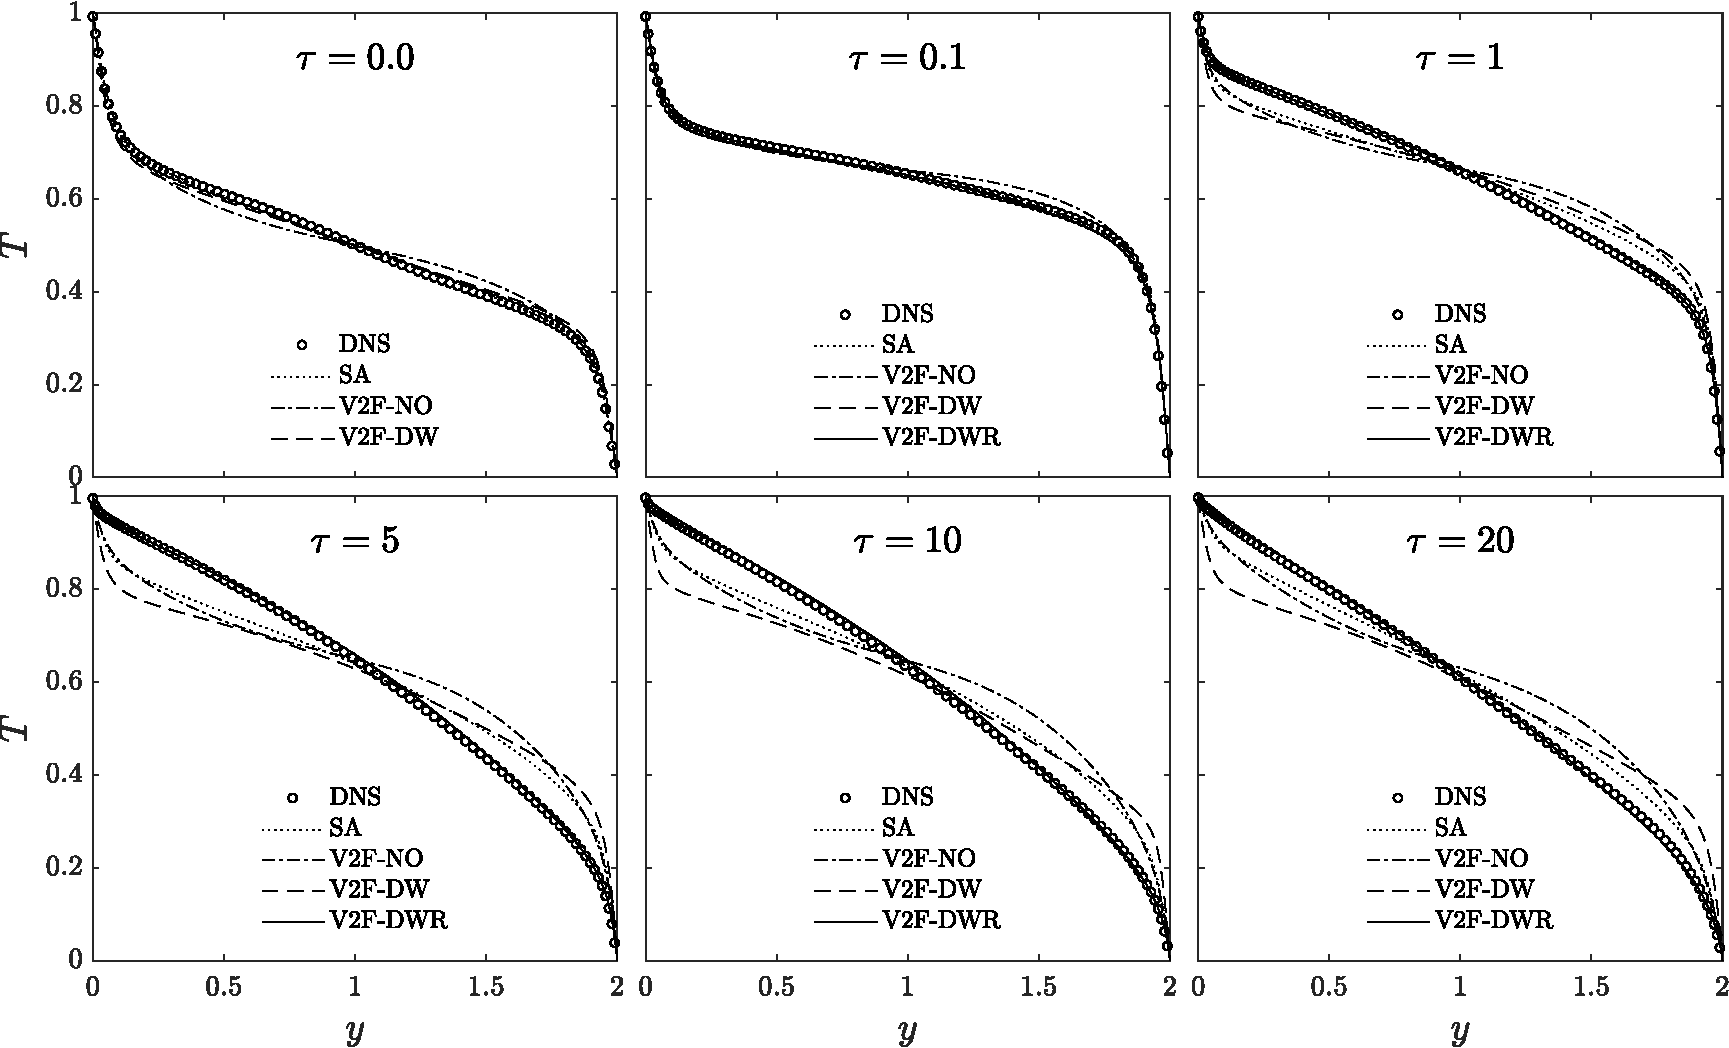
\includegraphics[width=1.1\textwidth]{../solution/Figures/Tempgrey.pdf}
\caption{\noindent RANS simulation with different turbulent heat flux models for different $\tau$ cases for constant density / constant absorption coefficient cases}
\label{constk}
\end{figure}

\begin{figure}[h]
\centering
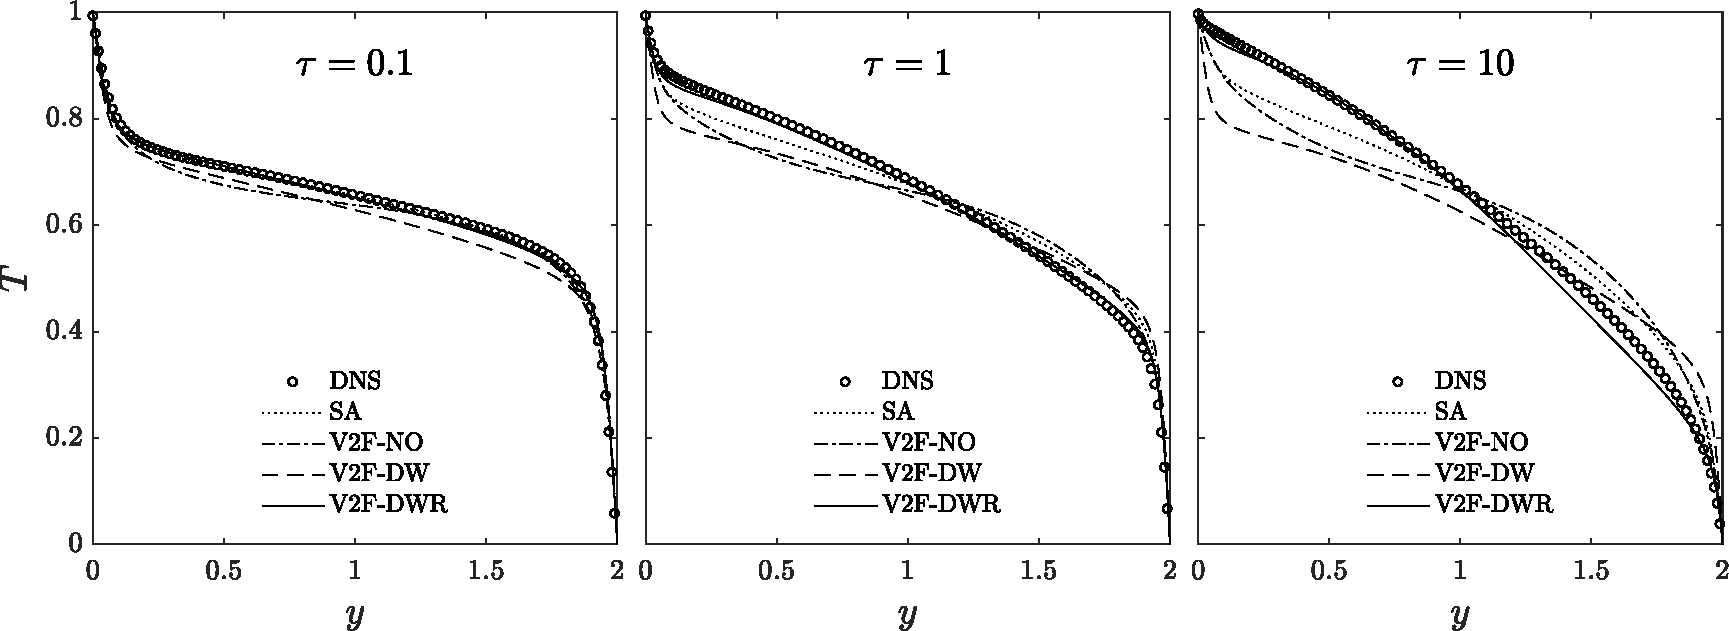
\includegraphics[width=1.1\textwidth]{../solution/Figures_r/Tempvar.pdf}
\caption{\noindent RANS simulation with different turbulent heat flux models for different $\tau$ cases or variable density / variable absorption coefficient cases}
\label{vark}
\end{figure}


\end{document}
